\documentclass[10pt,twocolumn,letterpaper]{article}
%% Welcome to Overleaf!
%% If this is your first time using LaTeX, it might be worth going through this brief presentation:
%% https://www.overleaf.com/latex/learn/free-online-introduction-to-latex-part-1

%% Researchers have been using LaTeX for decades to typeset their papers, producing beautiful, crisp documents in the process. By learning LaTeX, you are effectively following in their footsteps, and learning a highly valuable skill!

%% The \usepackage commands below can be thought of as analogous to importing libraries into Python, for instance. We've pre-formatted this for you, so you can skip right ahead to the title below.

%% Language and font encodings
\usepackage[english]{babel}
\usepackage[utf8x]{inputenc}
\usepackage[T1]{fontenc}

%% Sets page size and margins
\usepackage[a4paper,top=3cm,bottom=2cm,left=3cm,right=3cm,marginparwidth=1.75cm]{geometry}

%% Useful packages
\usepackage{amsmath}
\usepackage{graphicx}
\usepackage[colorinlistoftodos]{todonotes}
\usepackage[colorlinks=true, allcolors=blue]{hyperref}
\usepackage{natbib}
\bibliographystyle{unsrt}
%% Title
\title{
		\usefont{OT1}{bch}{b}{n}
		\normalfont \normalsize \textsc{UT Austin - Neural Networks Fall 2021} \\ [10pt]
		\huge Group 10: SuperTuxKart ice hockey \\
}
\selectlanguage{english}
\usepackage{authblk}
\author{Marlowe Johnson, Pedro Silva, Austin Aurelio, Luis Kaiser}

\begin{document}
\maketitle

\begin{abstract}
We present a deep learning residual network model (ResNet) with a dagger implementation as a base agent to successfully learn control policies for the state-based approach using reinforcement learning. The model is a ResNet, trained with the reinforce algorithm, whose input is the player and the soccer state, and the output is a value for braking, steering and accelerating. The DAGGER algorithm is used to pretrain our model imitating the Jurgen expert to provide a pre-trained base. The hyperparameters of all deep learning models were optimized separately using grid search. We find that our agent outperforms all provided agents on the local grader.  
\end{abstract} \\ 
\\ 
{\textbf{Keywords} \\
deep reinforcement learning, DAGGER, state based}

\section{Setup}
In the following, we are going to (i) discuss the model architecture and hyperparameters and (ii) explain the data generation.

\subsection{Model}
To ease the training of deep networks, we used a ResNet architecture with Mish activation function and 15 ResNet blocks with exponentially growing layer size to the power of two. As an input to our model, we extracted features of player state and puck state like Jurgen did in his code. The idea behind this was that since we use Jurgens agent as an expert, we should have the same inputs. Expanding the feature dimension, for example by including the opponent state, did not change the performance, but was especially more costly while training. Overall, the features tensor includes both kart centers, the kart angle, the kart to puck angle, the center of both goal lines, the difference between the kart angle and the kart to puck angle, both puck locations and the difference between the puck centers and both goal lines.

An extensive grid search is used to fine tune the hyperparameters. It follows that the Adam Optimizer with weight decay, a learning rate of .001 and a batch size of 512 achieves the best results while training. Using Dropout has proven to be helpful in our model architecture to better generalize, while adding a learning rate scheduler however did not improve the training progress. Changing the activation function from ReLU to Mish reduced the loss slightly.

For acceleration, we treated the problem as regression. We used the SmoothL1 loss function since this gave us the most stable training results. Any acceleration values outside of the range [0, 1] are clipped to 0 or 1. For steering and braking we treated the problem as a classification problem, we used the BCE with logits loss and progragated the outputs of the model through a sigmoid function to distribute the values from 0 to 1. Specifically for steering, the two possible classifications are 0, which we map to a steering of -1, and 1, which we map to a steering of 1. The sum of the individual losses is then back-propagated through the network. In terms of braking, our model brakes if the activation value is below 0.5, and does not if the value is above.

Since Jurgens algorithm uses only one model for both karts and we are imitating his policy, we decided to train only one neural network. On one hand, this results in a model that is easier and faster to train, while on the other hand it is not possible to train different policies.

\subsection{Data generation and Training}
For both learning algorithms, our data is generated in the training loop by letting our agent play against the provided agents from the teaching assistants (TA’s). Jurgen’s agent is used as an expert for DAGGER, as well as the opponent for deep reinforcement learning (DRL). Our model scored the fewest goals against Geoffrey’s agent, because of which we decided to change the distribution of the TA’s agents we play against.

For data augmentation and diversity, we used a random ball initialization and velocity of the puck. Since the puck starts at [0,0] after a goal is scored, our games only last one goal or till 1000 frames have passed. Furthermore, we randomly select the opponent for our agent to play against from a pool of agents consisting of the provided TA agents (Jurgen, Yoshua, Yann, etc.) as well as our own “dummy” agent which does not do anything. We found that including this additional “dummy” agent allowed our agent’s policy to quickly converge to one that is able to score goals. This is because against a “dummy” opponent, the agent is in a position where it’s only concern is to score a goal instead of having to consider positions where it may have to be defensive due to adversarial agents. Since the team id changes when grading, we switch sides after each epoch. This gives us more stable training results and a superior generalization.

Our training is done on colab with T4 and P100 GPUs. Overall, our final DAGGER algorithm took one hour to train, and the reinforcement learning optimization around half an hour.



\section{Development Process}

In recent years, different variants of DRL have become state-of-the-art for learning optimal strategies in video games. These successes motivate our approach to reinforcement learning. 

\subsection{Deep reinforcement learning approach}
In the early stages of our project, our goal was to implement a DRL agent that first trains by playing against the TA agents, and then plays against itself to surpass their performance. The initial reward function consisted of the distance between the puck and the goal, and the goals scored per game. Since the pitch is 64.5*2 long, we chose to reward our agent with 64.5*2 if he scores a goal; the distance is a float value of the distance. 

This simple setup did not learn as desired: The main reason was that after a couple of epochs, the model got stuck in corners and could not optimize its policy well enough to overcome these mistakes. Besides, games ended fast because the TA agents scored a goal quickly, not giving our agent enough time to explore the environment. Figure 1 shows two common failure scenarios while training. The first two pictures show the agent moving back and forth at their initial location. This behavior corresponds to the beginning of our training algorithm. The main reason for this is that the activations for braking and acceleration are almost random in the first epochs, which leads to a very unstable behavior and not enough exploration. The last two pictures correspond to the case where both agents steer heavily to the right and crash into the wall.

Therefore, in order to start training our reinforcement learning algorithm, we implemented a dummy agent that does not perform any actions. This has shown to be helpful to surpass some of the initial problems we had to get reinforcement learning to work, since our agent can now learn to drive towards the puck without interference. Furthermore, we changed the setup to only one agent playing which speeds up training time and makes the inputs to the model more similar.

The next step was to modify the reward function. The main issue with the initial approach of only using the distance between the puck and the goal was that the agent could not learn to first drive towards the puck to hit it towards the goal. By learning to drive towards the puck, the agent learns appropriate steering and acceleration to perform this simple task. Therefore, we began training the agent only with reward based on the distance between it and the puck. After that, we thought that adding the distance between the puck and the goal should give him the incentive to hit the puck from the right angle. After training for some time, it was clear that this approach would not work: The agent could not properly learn how to hit the puck to score a goal, and got confused when he hit the puck. We suspect that even with a sufficient reward function, it would take many many training iterations for the agent to learn a sensible policy. Our solution to this problem was to somehow provide a decent initialization to run reinforcement learning on top of. With a decent initialization, the agent would already know how to receive reward, and would easily be able to maximize it’s reward by improving it’s policy.

After looking through the class code, we then decided to implement a version of imitation learning algorithm to provide a DAGGER pre-trained network giving us a base we can further optimize with DRL.

\begin{figure}
  \centering
  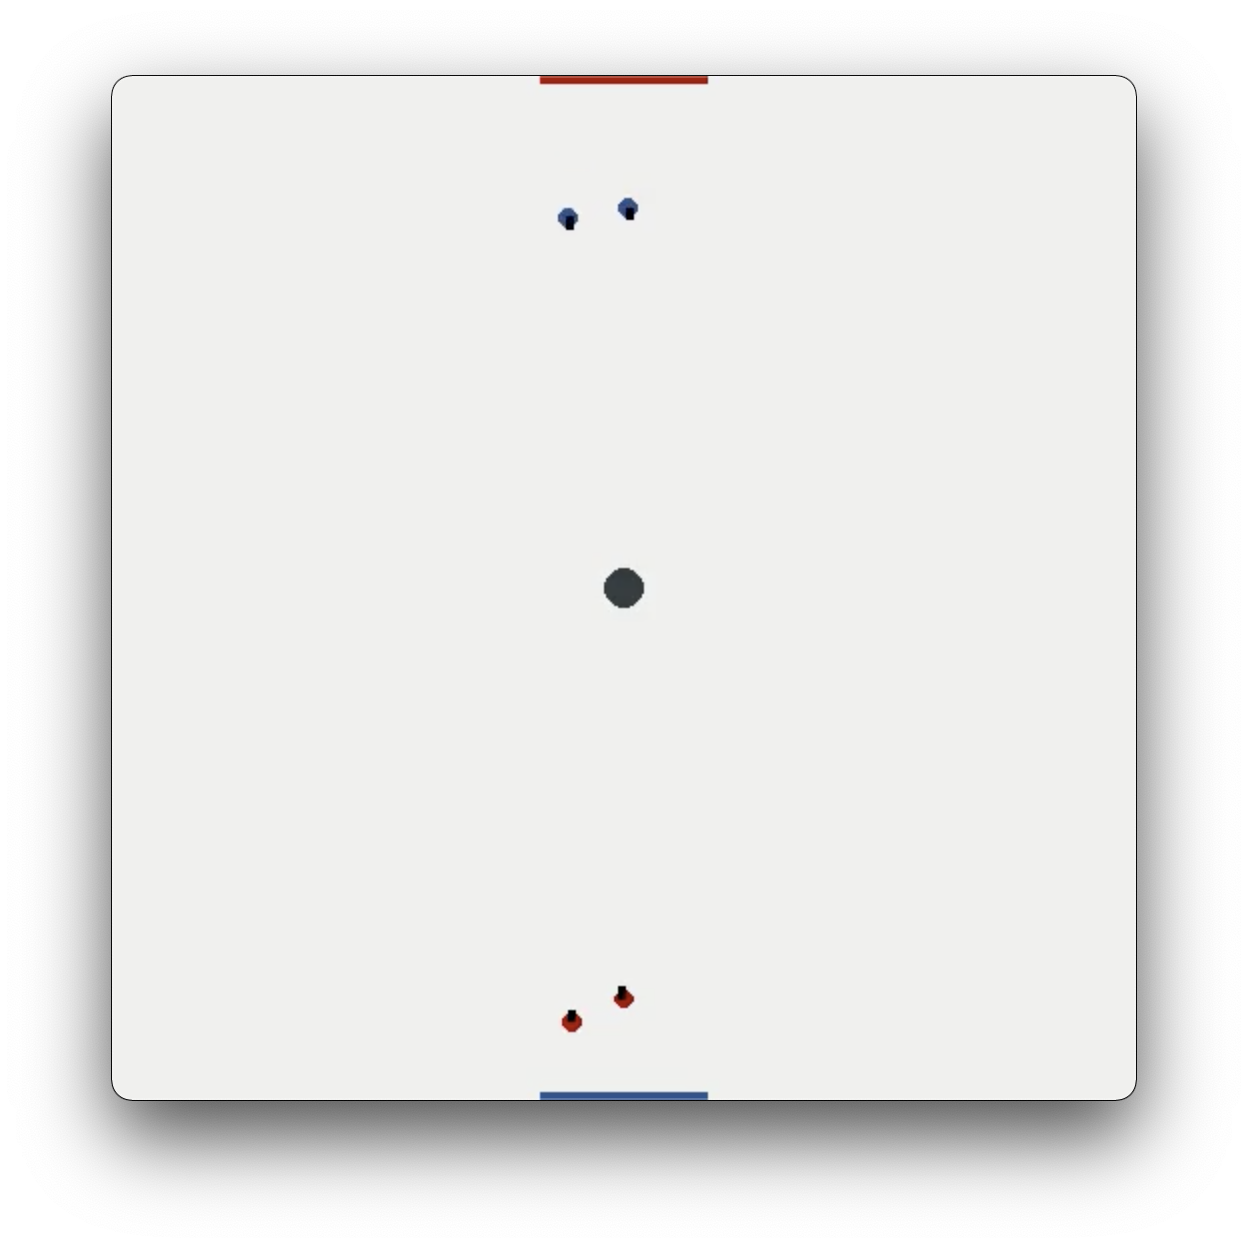
\includegraphics[width=0.24\textwidth]{figures/bf.png}
  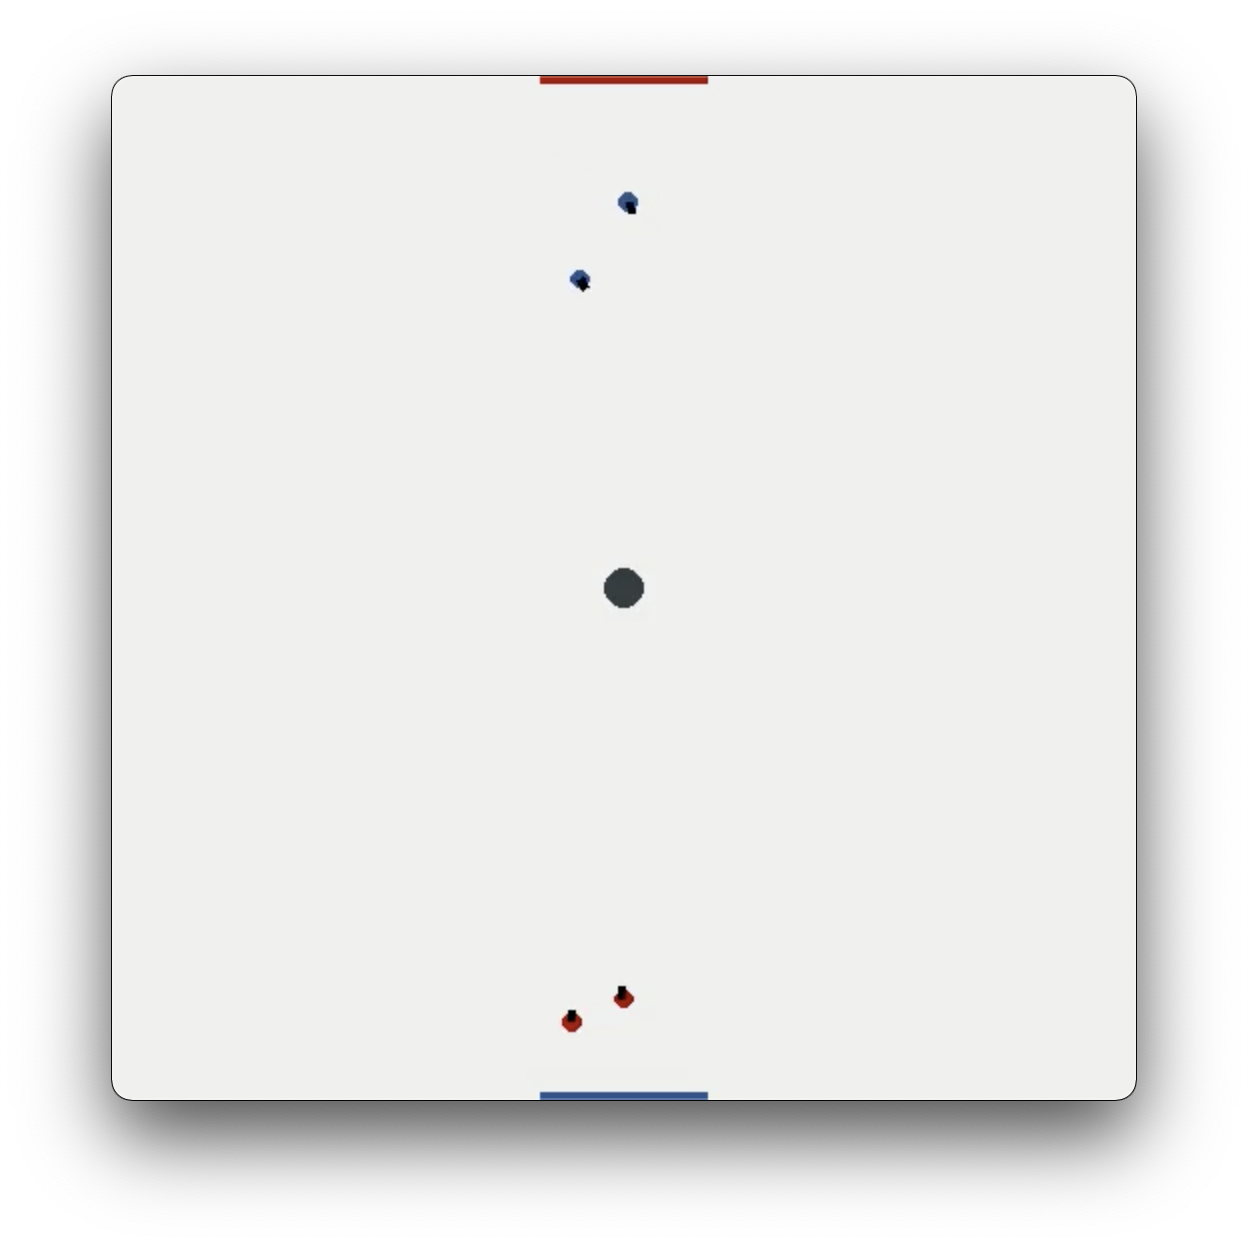
\includegraphics[width=0.24\textwidth]{figures/bf2.png}
  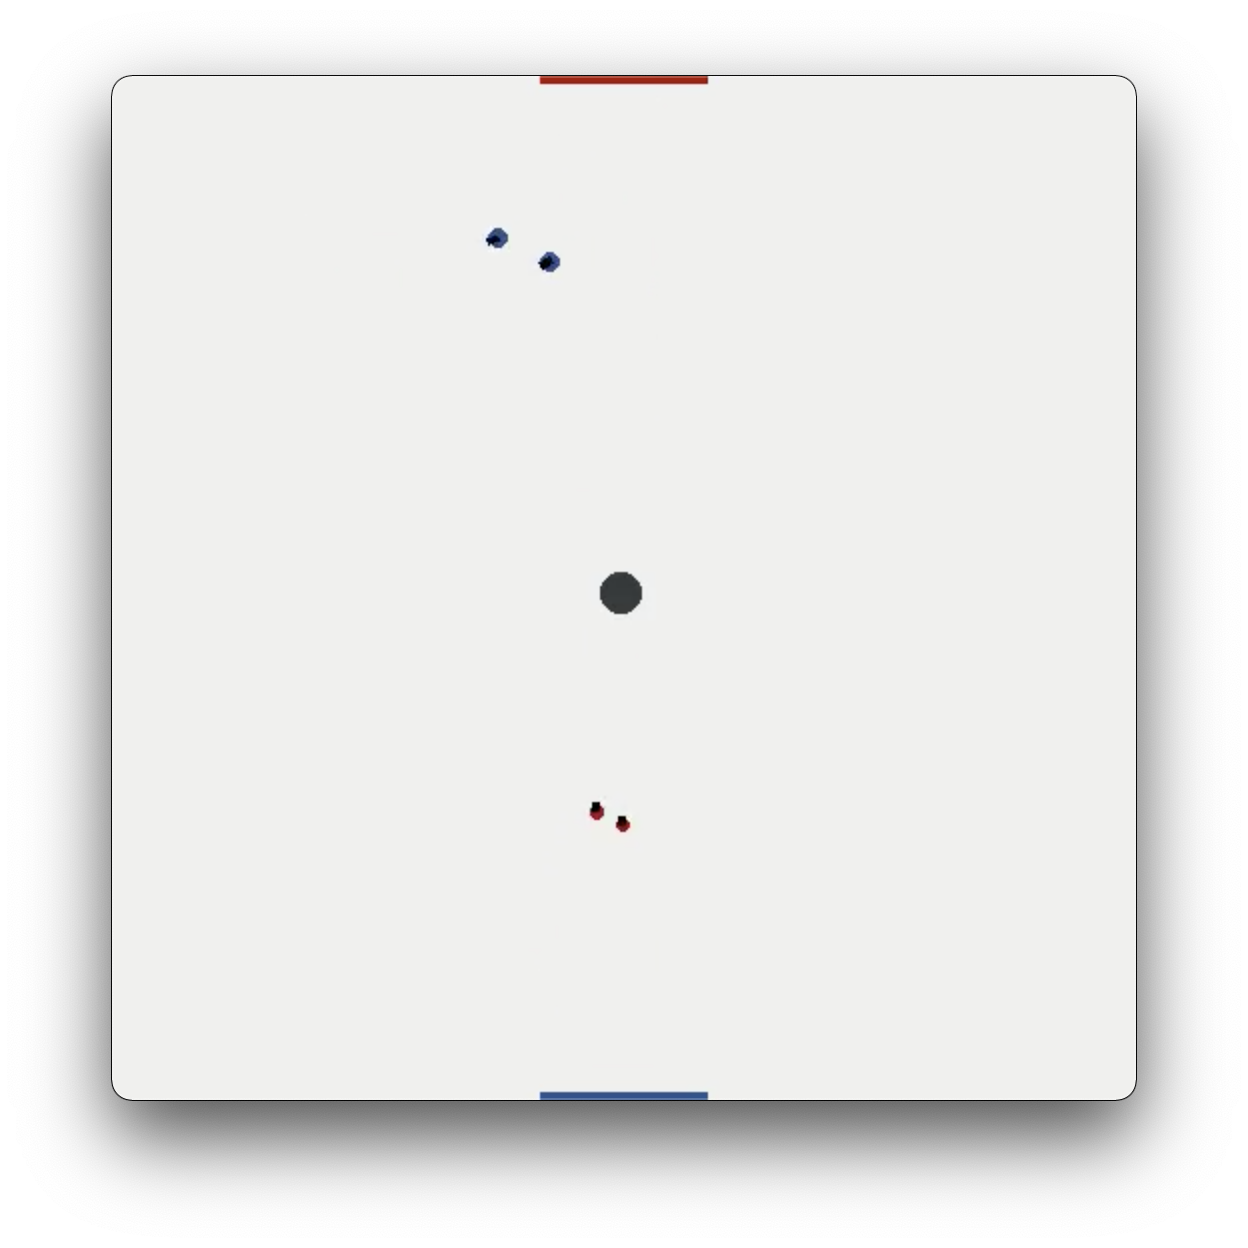
\includegraphics[width=0.24\textwidth]{figures/corner.png}
  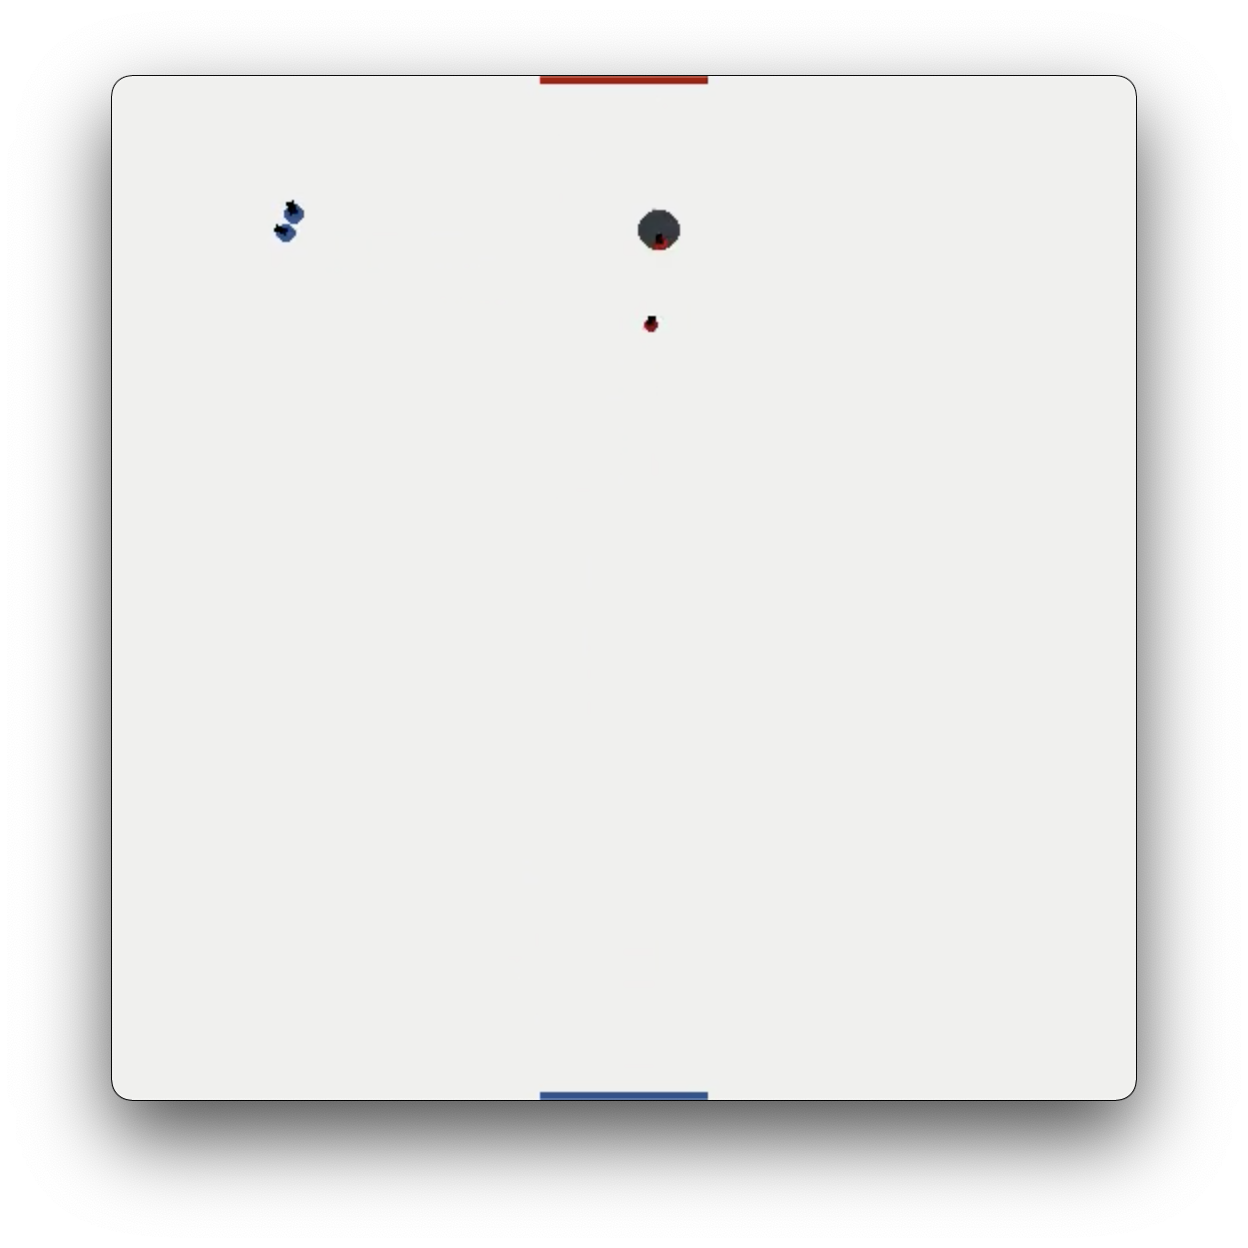
\includegraphics[width=0.24\textwidth]{figures/corner2.png}
  \caption{Example game state from the SuperTuxKart ice hockey with a state based agent using deep reinforcement learning. The blue agents (two karts on top of each pitch) use our model, while the red agents (two karts on the bottom) use Jurgens model. The images show two common failure cases when training the model with deep reinforcement learning.}
\end{figure}

\subsection{DAGGER}
In order to overcome mismatches in the training and testing distribution, we decided to implement DAGGER instead of vanilla imitation learning. The expert we imitated is Jurgen’s because he has proven to be the best in comparison to all other TA’s agents. For that reason, we used ‘sarah the racer’ as a kart to have the same setup as Jurgens algorithm.

For the first epoch, we allow the Jurgen expert to play a game, and collect the data it provides. Initially, we used our aforementioned “dummy” agent as the opponent for this first game because we wanted our agent to quickly learn to drive towards the puck and attempt to score a goal right at the beginning of the game. Once this behavior started to become apparent, we then randomized the opponents as mentioned before. The data for this initial game is saved into our dataset to be used in future epochs.

For the rest of the epochs, we begin to use DAGGER. Instead of having the Jurgen play the game, we allow our agent to play the game. For every state that our agent encounters, we collect the action that Jurgen would have done. We append this new data into our dataset to be used in future epochs.

As we continue training the agent, our data is aggregated in our dataset and we use random batches to shuffle our data. This leads to an unstable behavior of the loss in the beginning of the training loop, and a convergence to a value around .17 after 200 epochs. We noticed that our loss plateaus first at 1.3, and then drops remarkably after around 20 epochs. This led us to modify the hyperparameters such as the learning rate (i.e. scheduling), the optimizer and the batch size, as well as the model architecture including the hidden layer size and the activation function. Besides, we noticed that the model begins to win more than half of the games after the loss is below .2.

In Figure 2, we can see the progress and behavior of our DAGGER model when playing against Jurgen’s agent. The pictures indicate that the model is able to successfully steer behind the ball and hit it at a good angle. In addition, the last two pictures show that the model proves to be robust in unusual scenarios, e.g. the opponents are closer to our own goal than we are, or the ball is not in the center.

After 200 epochs, the performance of our model did not improve much; therefore, we continued improving our DAGGER-trained model by switching to DRL for further optimization as described in class.

\begin{figure}
  \centering
  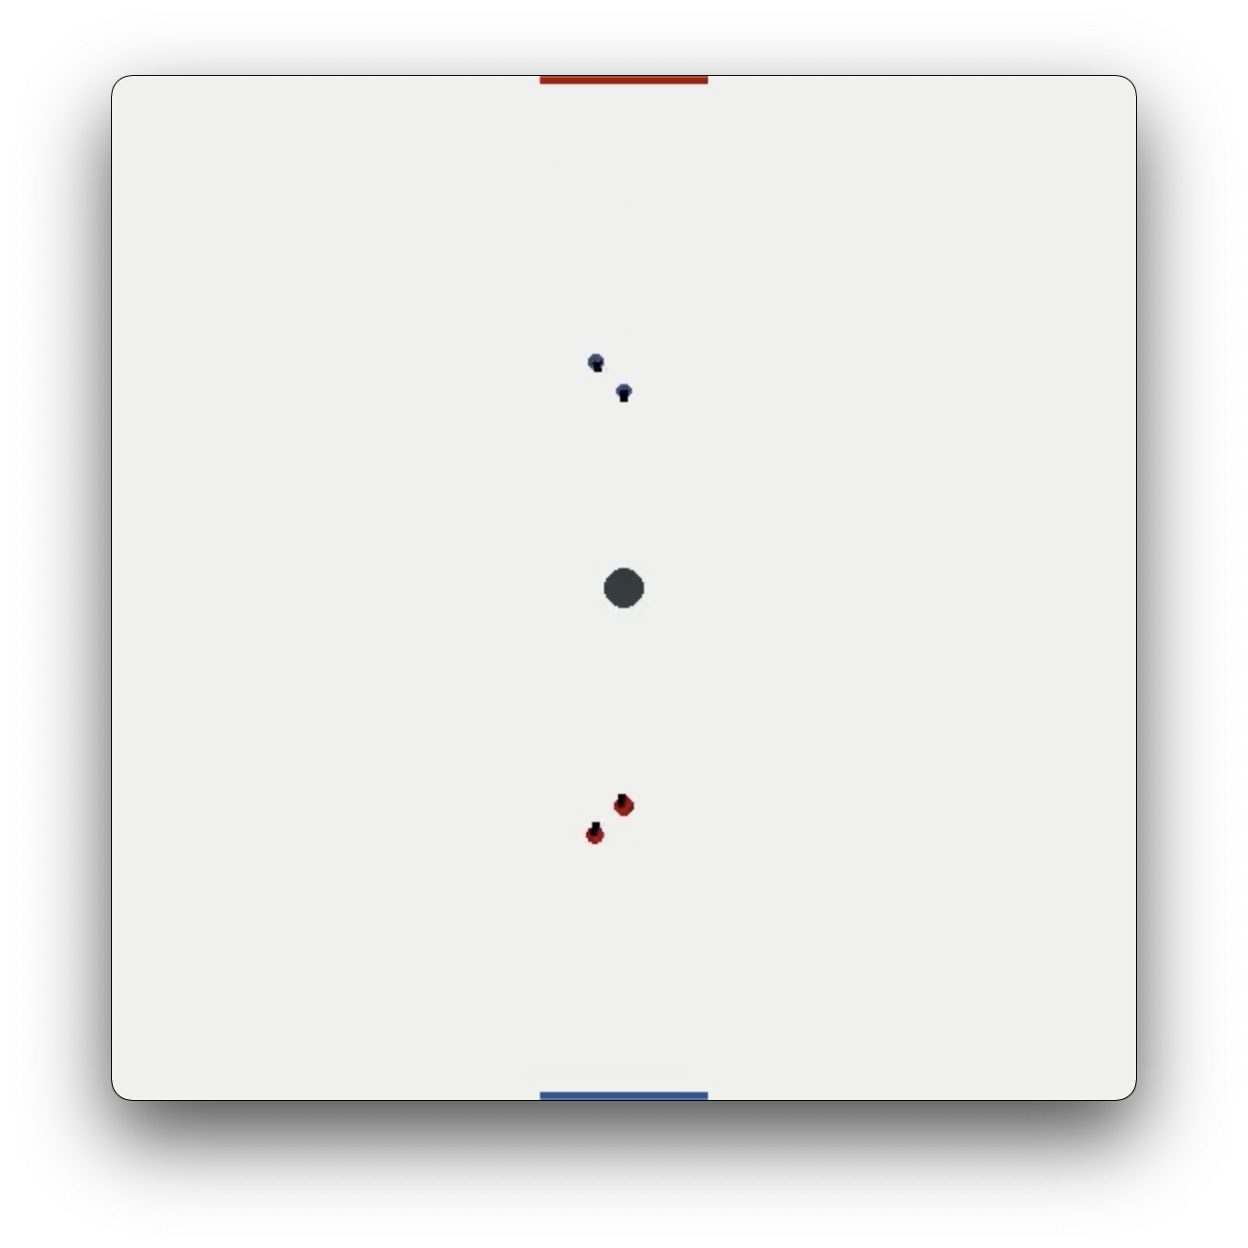
\includegraphics[width=0.4\textwidth]{figures/dagger_good.png}
  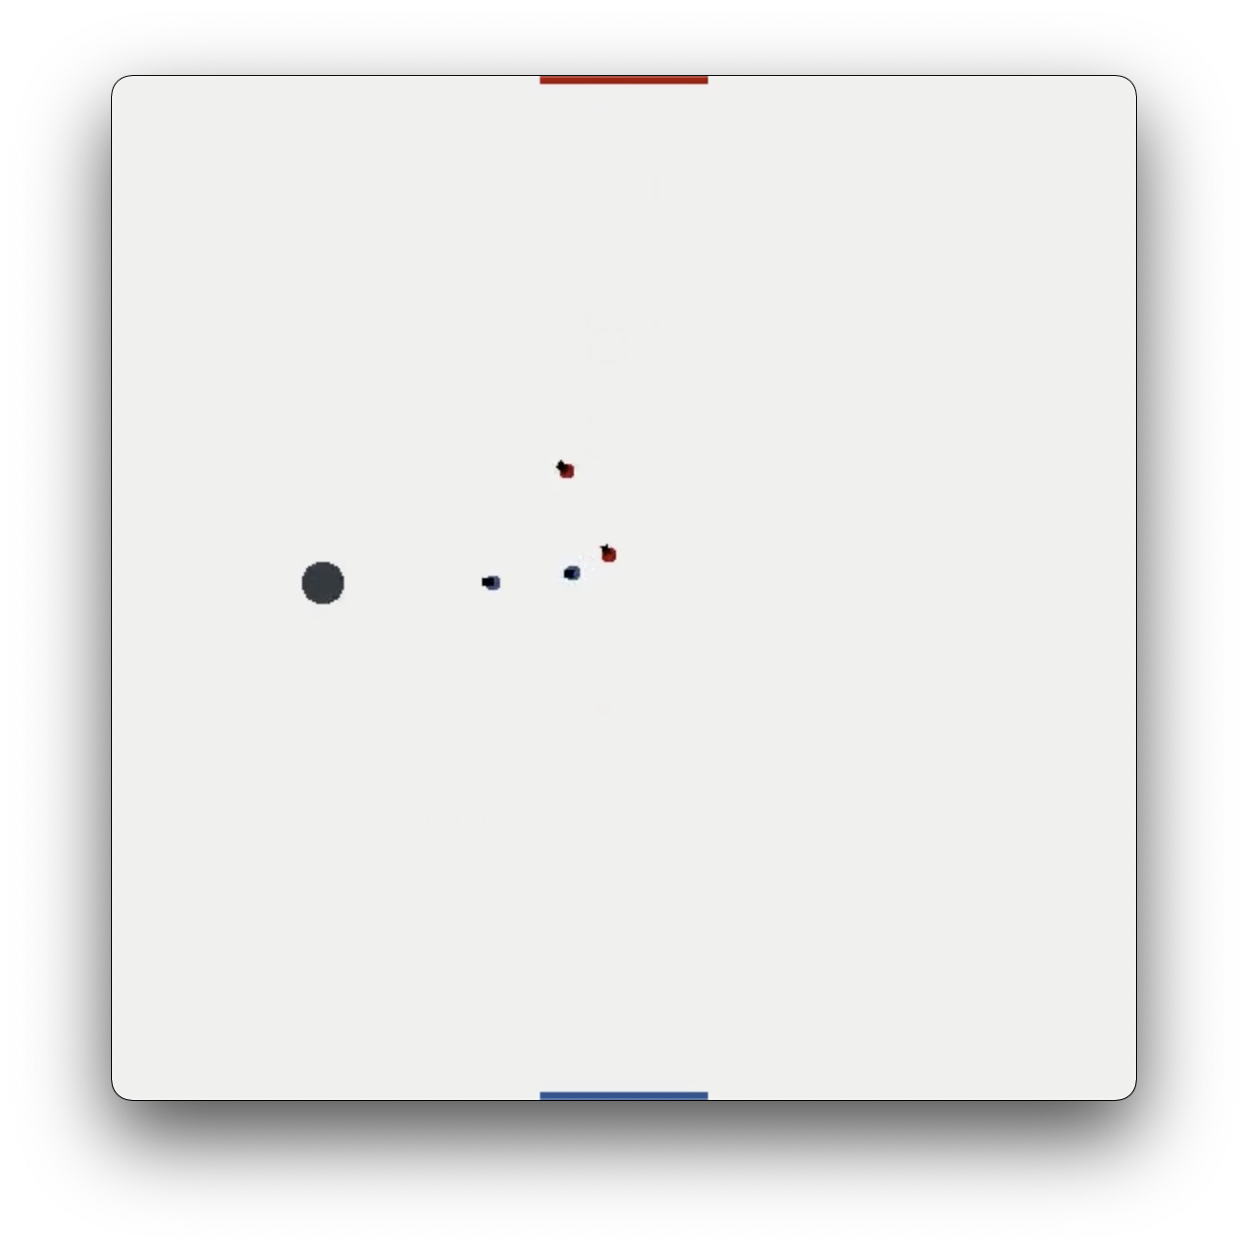
\includegraphics[width=0.4\textwidth]{figures/dagger_good3.png}
  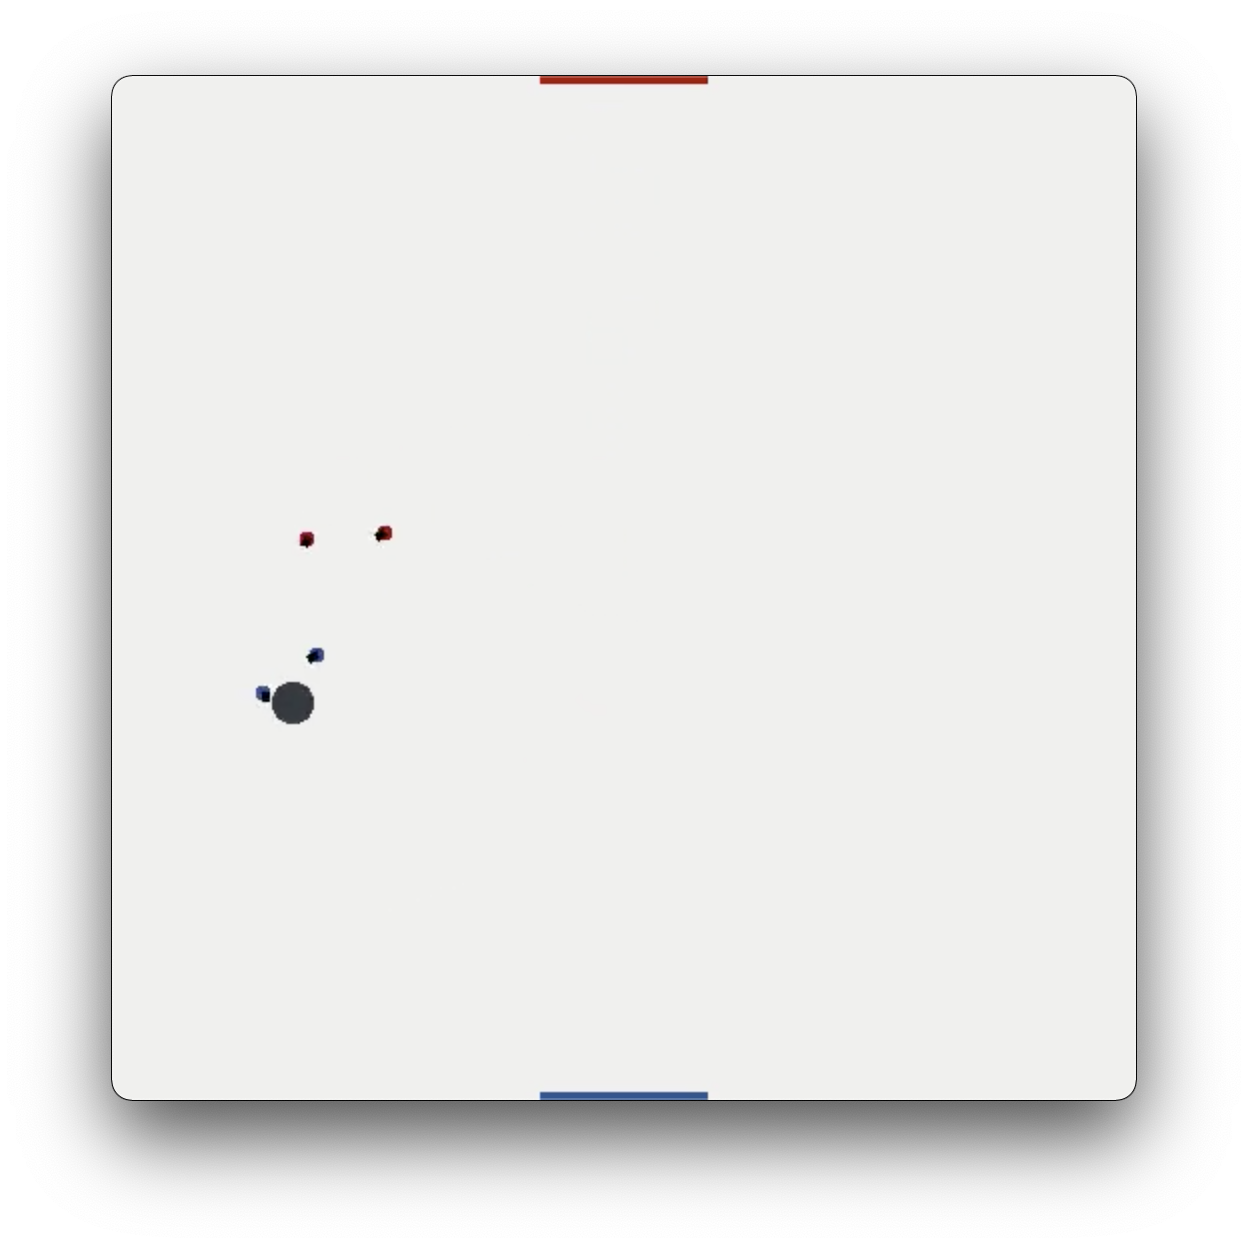
\includegraphics[width=0.4\textwidth]{figures/dagger_good2.png}
  \caption{Example game state from the SuperTuxKart ice hockey with a state based agent using the DAGGER algorithm. The pictures show the improvement to Figure 1, especially the successfull steering and align of the kart with the puck and the center of the goal line.}
\end{figure}

\subsection{Combining DAGGER and deep reinforcement learning}

The main idea was that using DRL, our agent could potentially learn to be better than the expert (Jurgen) it imitated. We first let our model play against Jurgen’s agent. For our reward function, we decided not to include the puck distance as our agent already knew to drive up to the puck. We chose to give rewards based solely on the goals as this is what we want to optimize, while keeping the policy simple.

After some iterations of DRL, we found that the agent did not improve all that much and sometimes even became worse. We believe that the problem is that giving rewards only based on goals scored is too general for the agent to learn anything useful. This is why we gradually changed the reward function as described above without any remarkable improvements. Perhaps a better reward function would have yielded better results in addition to using a modification to reinforce such as PPO or Q-learning.

Another hypothesis as to why reinforcement learning did not help our imitation learning agent is because it causes divergence from the learned policy. Because our training examples during imitation learning are frame-by-frame, the policy is learned based only on the current state and is not aware of a concept of reward in the future. 

\section{Discussion}

Our model can be further optimized in many different ways. First, we could do random search, instead of grid search, to fine tune the hyperparameters of our model. This would definitely improve our models performance, leading to a better and more stable training progress. By making the model deeper, e.g. adding more ResNet blocks, this may allow us to input more features to our model. However, we found out that having a larger model exceeds the allowed file size on Canvas. Second, playing against further agents would obviously improve our reinforcement learning agent. E.g. by implementing an evolutionary agent, we would have an additional agent we can play against, which uses another training algorithm than all previous agents. Using the evolutionary learning model as a base, or further optimizing our final model could have improved the performance.

Regarding optimizations for DRL, different reward functions enable the karts to learn multiple policies; one agent could be rewarded for playing more defensively, e.g. hitting the puck away from our own goal or being punished for receiving goals, while the other agent focuses on scoring goals. Another way to approach this issue is to first train the DAGGER algorithm with the “dummy” agent, and then use reinforcement learning to optimize the policy. This can then be done similarly for playing against the TA’s agents.

During training DAGGER, we ran into resource distribution problems: We could not run a match on the GPU, so we decided to train on CPUs. However, this would lead to time outs on the grader. After a lot of debugging, we found out that the problem was that the model has a warm up period during the first call to forward after it is loaded from a .pk file. Because of this, the first call to our act function was timing out, and there was some logging code in the check function that used division by the iteration number. Because this was the first call to act, we were getting a division by zero error. Eventually we found out that if we ignored this logging by setting the iteration number to 1, the training would work fine on the GPU or CPU.

\section{Summary}
This paper introduced our DAGGER base model and a DRL algorithm to master difficult control policies for the SuperTuxKart ice hockey computer game using states as an input. We have presented the hyperparameter selection for our model architecture and setup, as well as the obstacles we encountered during training. We have explained our solutions and discussed further optimizations.

\end{document}
